\documentclass{article}
\usepackage[UTF8]{ctex}
\usepackage{geometry}
\usepackage{listings}
\usepackage{subfigure}
\usepackage{float}
\usepackage{fancyhdr}
%\usepackage[colorlinks,linkcolor=blue]{hyperref} 

%\usepackage{amsmath}
\usepackage{graphicx}
%\usepackage{pgfplots}

\geometry{left = 2cm,right = 2cm,top = 3cm,bottom = 3cm}
\pagestyle{fancy}
\fancyhf{}
\fancyhead[R]{\leftmark}
\fancyhead[L]{\rightmark}
\fancyhead[C]{预习报告}
\fancyfoot[C]{\thepage}
\renewcommand{\headrulewidth}{0.2mm}

\title{预习报告}

\author{王晨宇 孙博然}

\begin{document}

\maketitle

\section{发送电路}
\subsection{电路图}
电路初步设计如图所示
\begin{figure}[H]
    \centering
    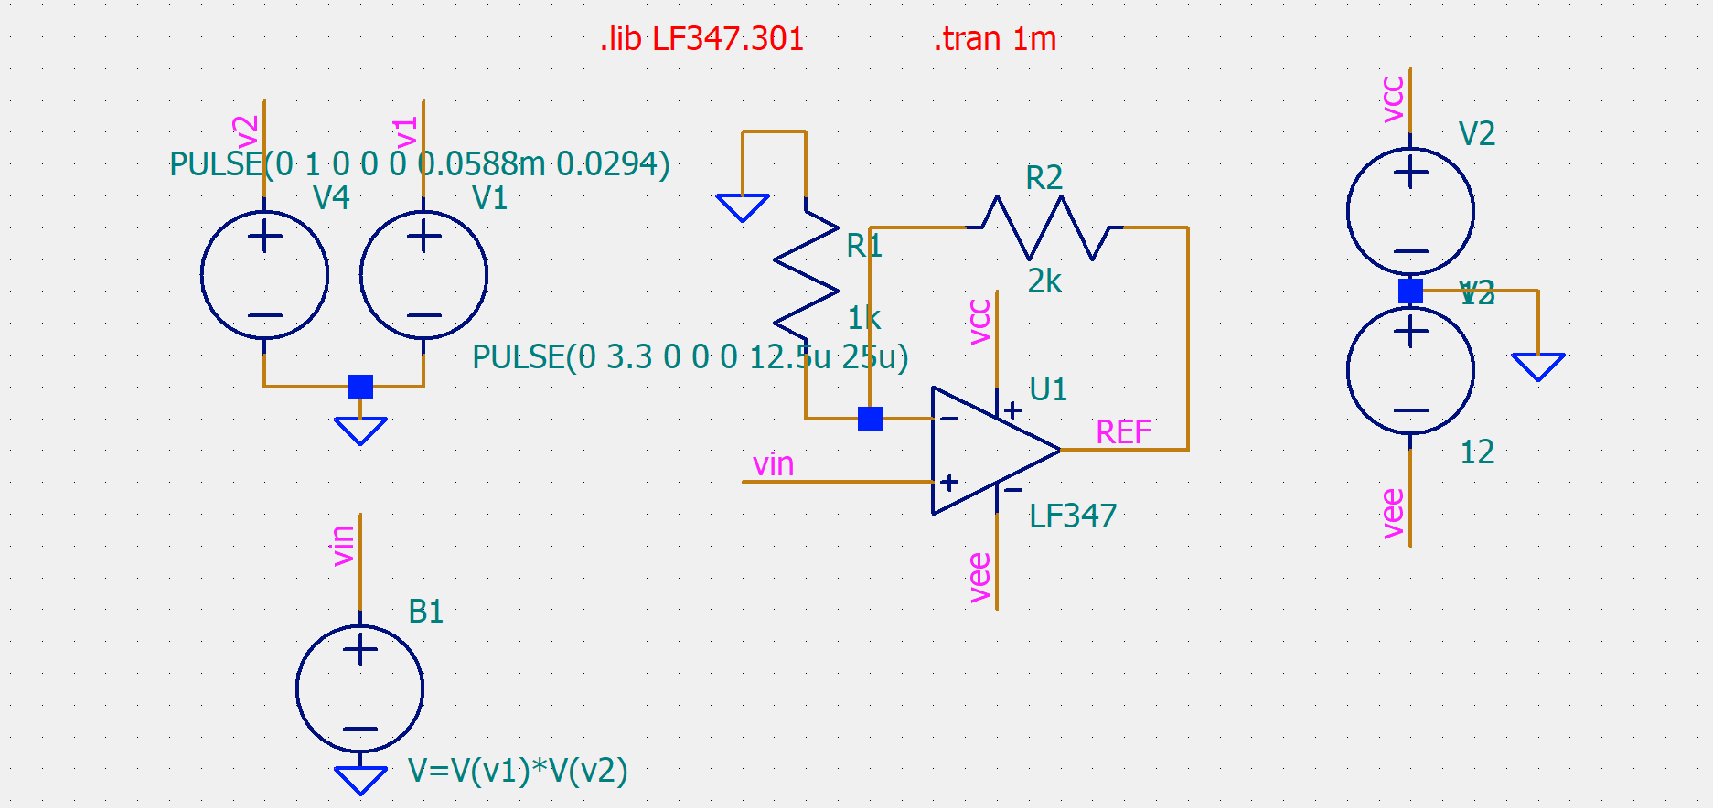
\includegraphics[width = 12cm]{images/tx_cir.png}
    \caption{发送电路图}\label{fig1}
\end{figure}
采用摆率较大的LF347放大器,同相放大,放大倍数设置为3。LF347需要接10V电源。
\subsection{仿真结果}
\begin{figure}[H]
    \centering
    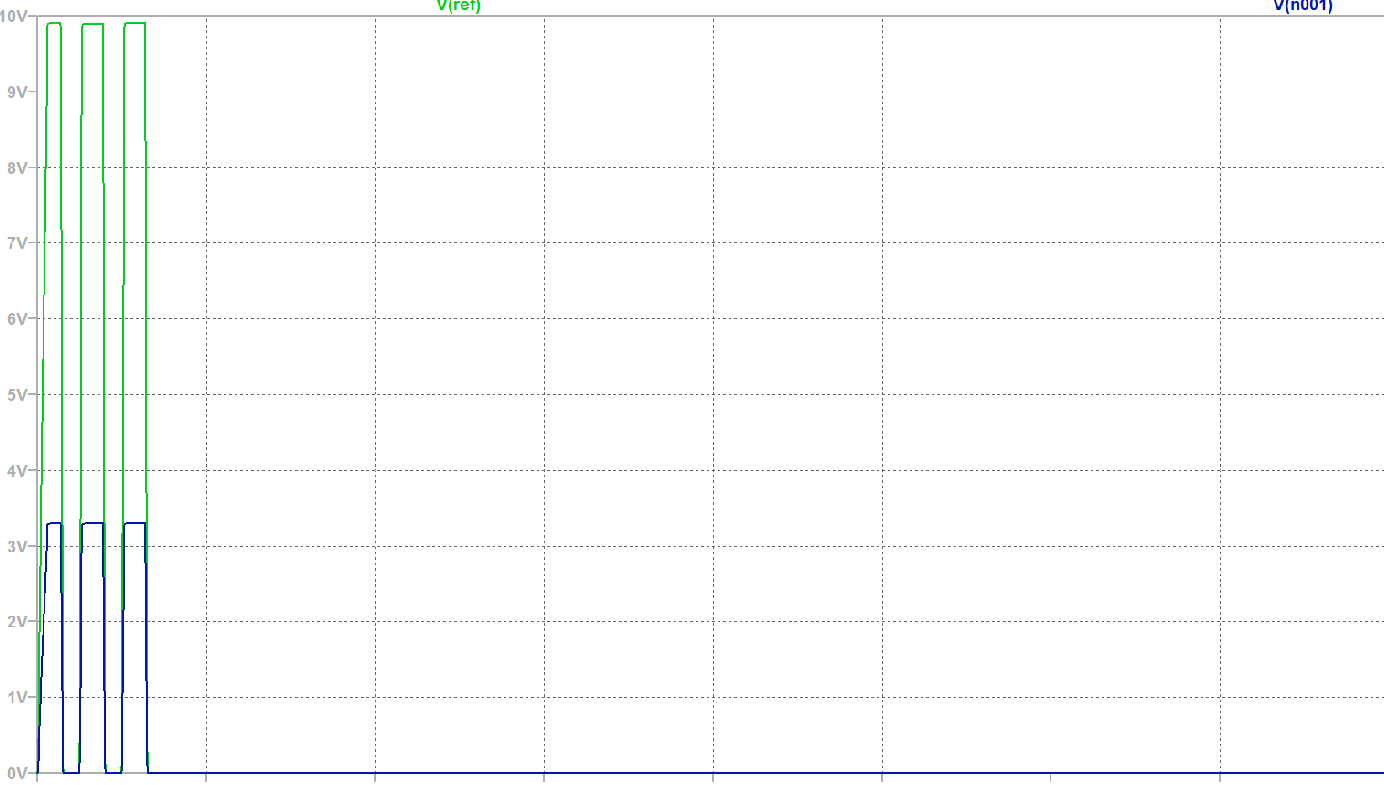
\includegraphics[width = 12cm]{images/tx_waveform.png}
    \caption{发送电路仿真结果}\label{fig2}
\end{figure}

\section{接收电路}
如图所示
\begin{figure}[H]
    \centering
    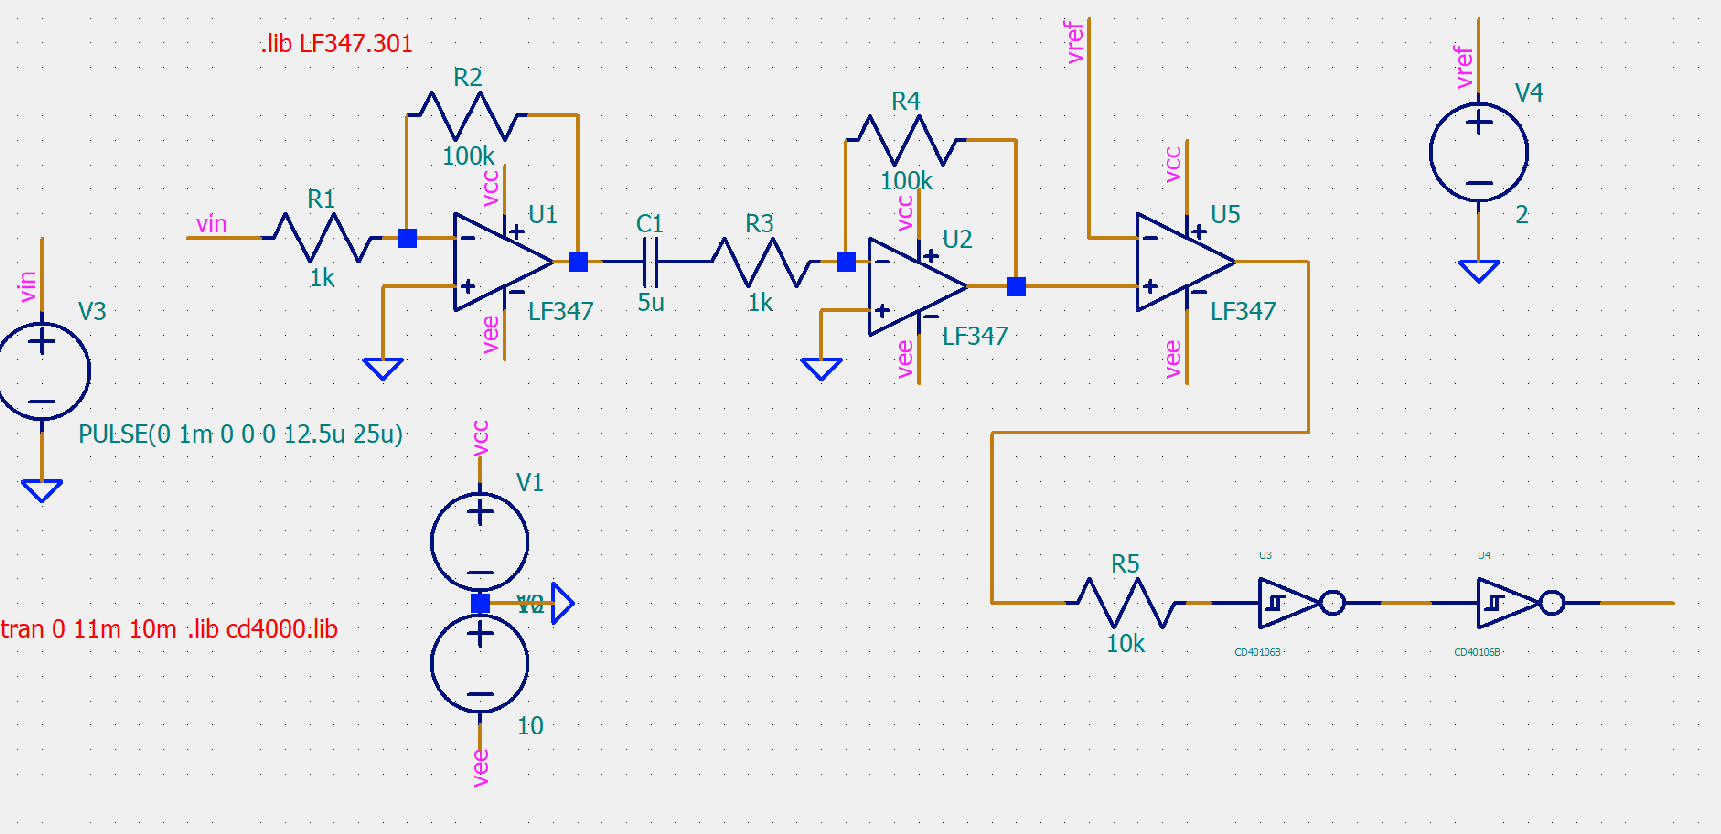
\includegraphics[width = 12cm]{images/rx_cir.png}
    \caption{接收电路图}\label{fig3}
\end{figure}
考虑到增益LF347增益带宽积,采用两级反相放大,中间添加电容去除直流分量。比较器Vref暂时定位2V,之后连接匹配整形电路。
\subsection{仿真结果}
\begin{figure}[H]
    \centering
    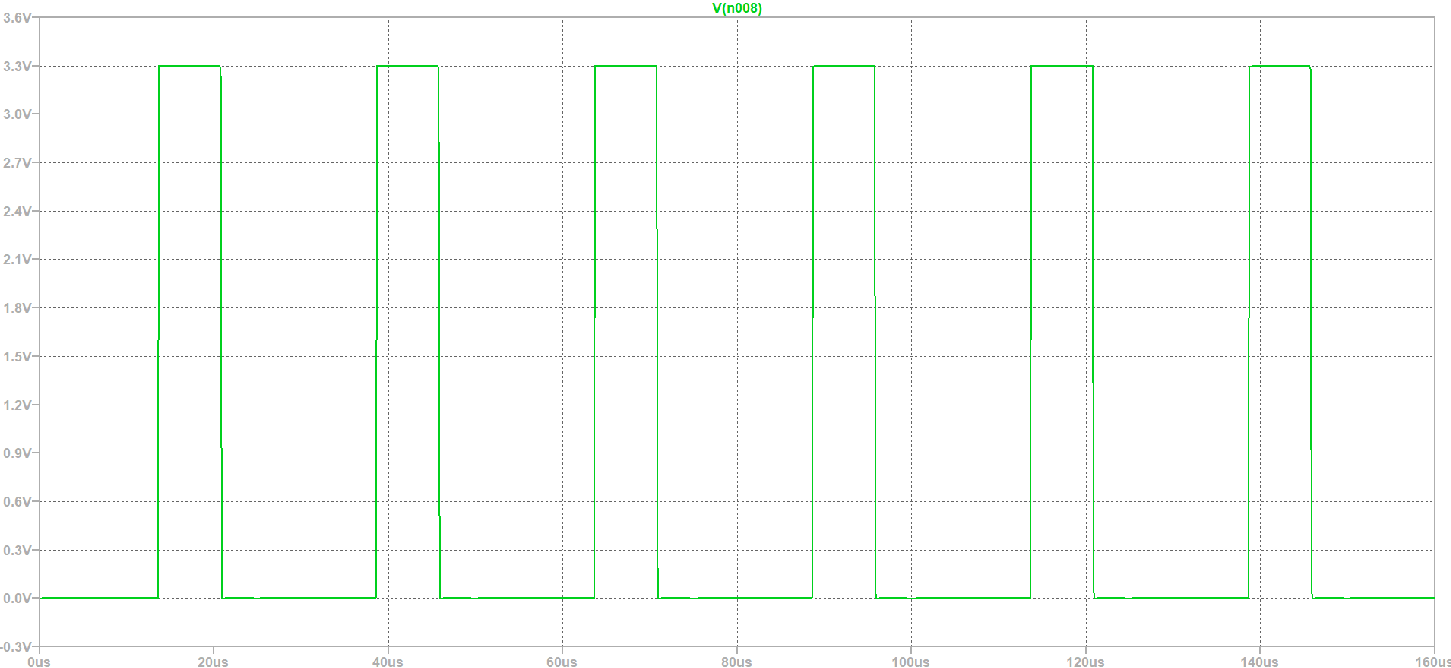
\includegraphics[width = 12cm]{images/rx_waveform.png}
    \caption{接收电路仿真结果}\label{fig4}
\end{figure}
CD40106饱和电压设置3.3V(与fpga相连接)。

\section{脉冲产生、计数与显示}
\subsection{电路图}
\begin{figure}[H]
    \centering
    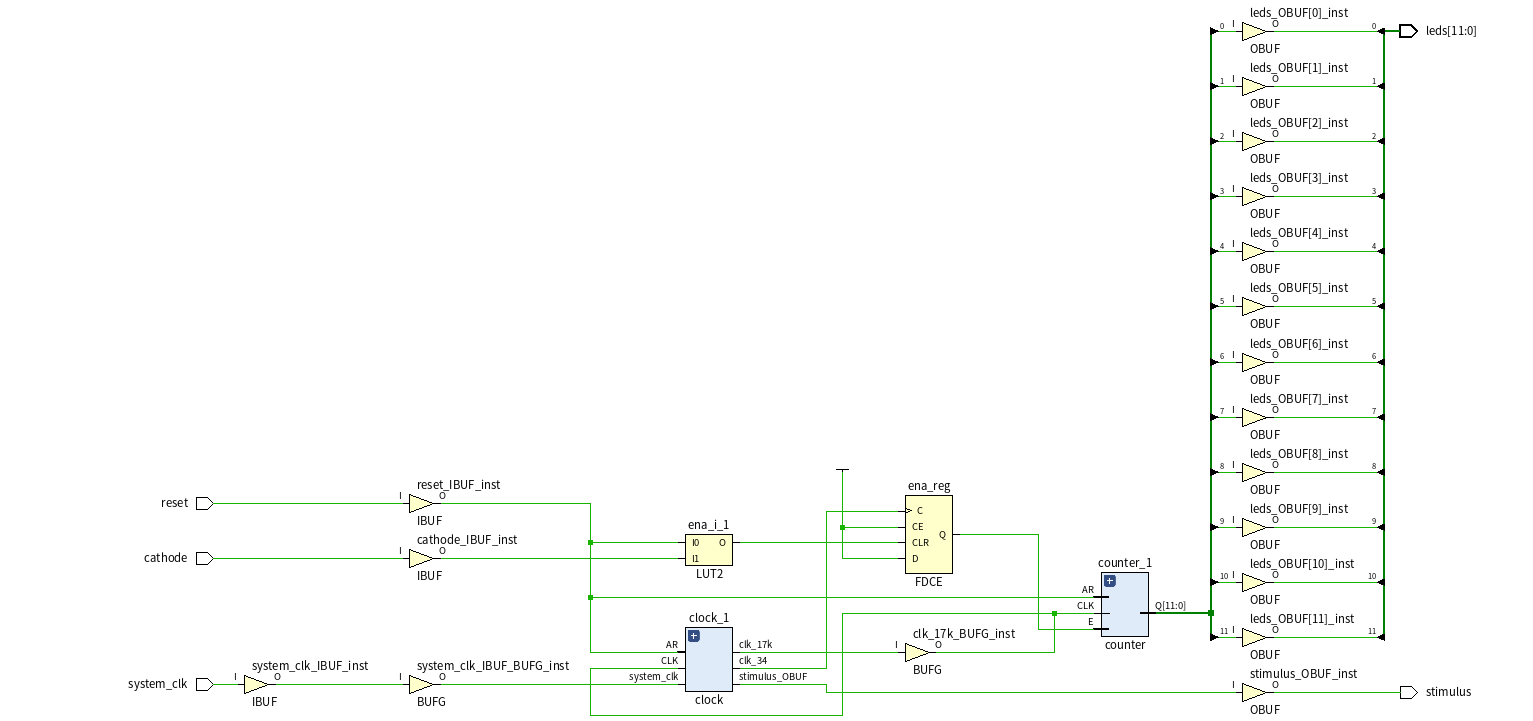
\includegraphics[width = 12cm]{images/schematic.png}
    \caption{脉冲产生、计数与显示电路}\label{fig5}
\end{figure}
\subsection{仿真结果}
\begin{figure}[H]
    \centering
    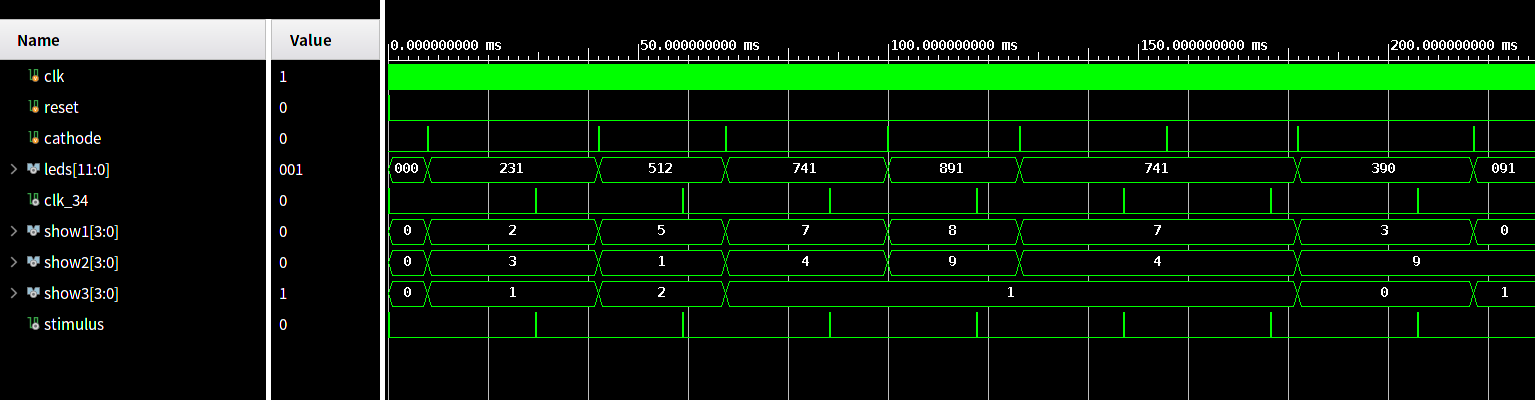
\includegraphics[width = 12cm]{images/timing.png}
    \caption{仿真结果}\label{fig6}
\end{figure}
%\begin{lstlisting}[language=Matlab]
%\end{lstlisting}

\end{document}